\documentclass[tikz,border=6pt]{standalone}
\usepackage{times}
\usetikzlibrary{positioning,arrows.meta,fit,backgrounds}
\tikzset{
  stage/.style={draw, line width=0.5pt, rounded corners=1.5pt, align=left, inner sep=6pt, minimum height=24mm, text width=40mm, font=\small},
  group/.style={draw, line width=0.5pt, rounded corners=2pt, inner sep=6pt},
  grouplabel/.style={font=\small\bfseries, anchor=south west},
  flow/.style={-{Latex[length=2.2mm]}, line width=0.6pt},
  edgelabel/.style={font=\footnotesize, fill=white, inner sep=1.5pt},
  title/.style={font=\small\bfseries},
}
\begin{document}
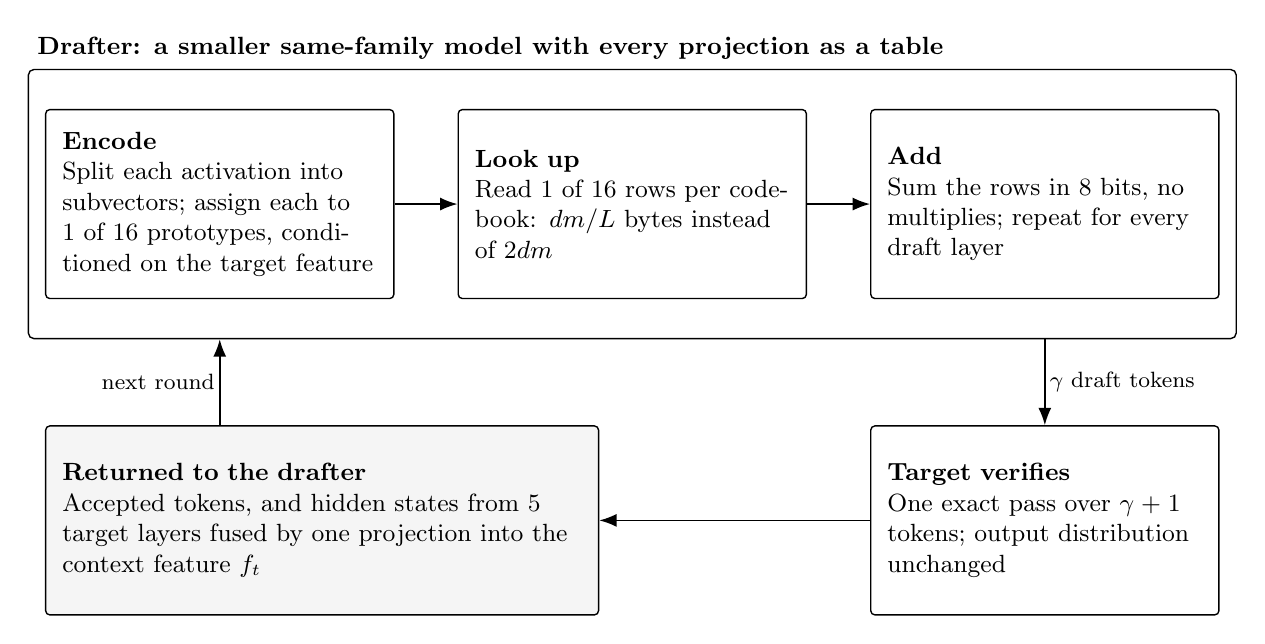
\begin{tikzpicture}
  % drafter stages
  \node[stage] (enc) {\textbf{Encode}\\Split each activation into subvectors; assign each to 1 of 16 prototypes, conditioned on the target feature};
  \node[stage, right=8mm of enc] (look) {\textbf{Look up}\\Read 1 of 16 rows per codebook: $dm/L$ bytes instead of $2dm$};
  \node[stage, right=8mm of look] (add) {\textbf{Add}\\Sum the rows in 8 bits, no multiplies; repeat for every draft layer};
  \draw[flow] (enc) -- (look);
  \draw[flow] (look) -- (add);
  \begin{scope}[on background layer]
    \node[group, fit=(enc)(look)(add), label={[grouplabel]north west:Drafter: a smaller same-family model with every projection as a table}, inner ysep=5mm] (drafter) {};
  \end{scope}
  % verify and return
  \node[stage, below=16mm of add.south, anchor=north, text width=40mm] (ver) {\textbf{Target verifies}\\One exact pass over $\gamma+1$ tokens; output distribution unchanged};
  \node[stage, text width=66mm, fill=black!4] (ret) at (ver -| enc.west) [anchor=west] {\textbf{Returned to the drafter}\\Accepted tokens, and hidden states from 5 target layers fused by one projection into the context feature $f_t$};
  \draw[flow] (drafter.south -| add) -- (ver.north) node[edgelabel, midway, right] {$\gamma$ draft tokens};
  \draw[flow] (ver.west) -- (ret.east);
  \draw[flow] (ret.north -| enc) -- (drafter.south -| enc) node[edgelabel, midway, left] {next round};
\end{tikzpicture}
\end{document}
